%% Beispiel-Präsentation mit LaTeX Beamer im KIT-Design
%% entsprechend den Gestaltungsrichtlinien vom 1. August 2020
%%
%% Siehe https://sdqweb.ipd.kit.edu/wiki/Dokumentvorlagen

%% Beispiel-Präsentation
\documentclass[en]{sdqbeamer}
 
%% Titelbild
\titleimage{unima_schloss}

%% Gruppenlogo
\grouplogo{} 

%% Gruppenname und Breite (Standard: 50 mm)
\groupname{Mannheim Master Datascience}
%\groupnamewidth{50mm}

% Beginn der Präsentation

\title[HybridBERT4Rec]{HybridBERT4Rec: A Hybrid Recommender System Based on BERT}
\subtitle{Sequential Content-Based and Collaborative Filtering}
\author[Leon Knorr]{Leon Knorr}

\date[\today]{\today}

% Literatur 
 
\usepackage[citestyle=numeric,bibstyle=numeric,hyperref,backend=biber]{biblatex}
\addbibresource{sources.bib}
\bibhang1em

\begin{document}
 
%Titelseite
\KITtitleframe

%Inhaltsverzeichnis
\begin{frame}{Table of Contents}
\tableofcontents
\end{frame}

\section{An Introduction to Sequential Content Recommendation}

\begin{frame}{Traditional CBF VS Sequential CBF}
	\begin{columns}
	\column{0.5\textwidth}
		\begin{figure}
			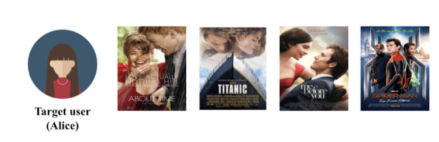
\includegraphics[width=\textwidth]{images/Alice_history.pdf}
			\caption{Example history for Alice in traditional CBF \cite{channarongHybridBERT4RecHybridContentBased2022}}
		\end{figure}
		\begin{itemize}
			\item models \textbf{general} user preference \pause
			\item \textbf{BUT:} User preferences \underline{\textbf{change over time!}} \cite{wangSequentialRecommenderSystems2019}
		\end{itemize}

	\column{.5\textwidth}
		\begin{figure}\pause
			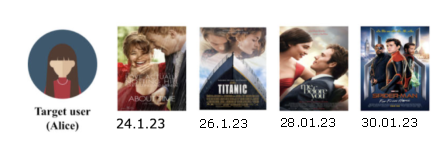
\includegraphics[width=\textwidth]{images/Alice_seq.pdf}
			\caption{Example history for Alice in sequential CBF \cite{channarongHybridBERT4RecHybridContentBased2022}}
		\end{figure}
		\begin{itemize}
			\item Considers the \textbf{order} of historical interactions
			\item Allows the modelling of \enquote{temporary spikes} of interests, as well as the general preferences \cite{wangSequentialRecommenderSystems2019}
		\end{itemize}
	\end{columns}
\end{frame}

\begin{frame}{A Common Approach to Sequential modelling}
	\begin{figure}
		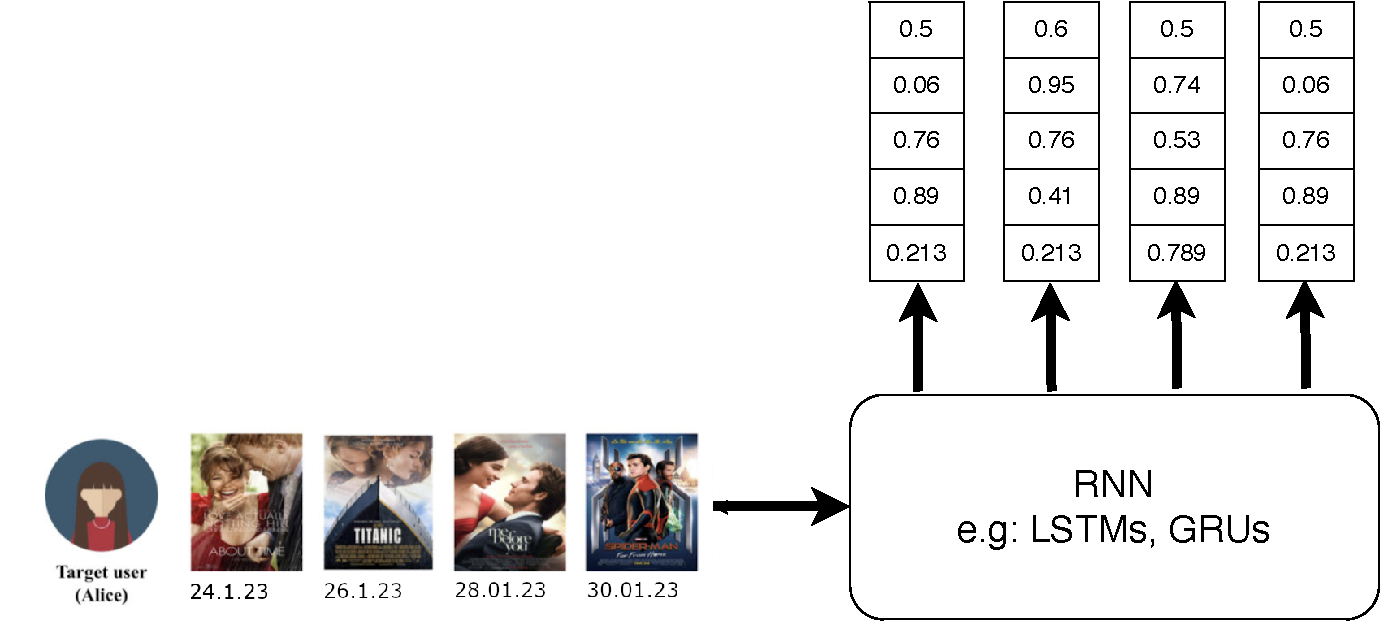
\includegraphics[height=0.45\textheight]{images/rnn_seq.pdf}
		\caption{Sequential Content Recommendation with RNNs. \cite{yuDynamicRecurrentModel2016}}
	\end{figure}
	\begin{itemize}
		\item Suffers from common RNN problems! Especially: \textbf{Catastrophic forgetting}, uni-directionality \cite{channarongHybridBERT4RecHybridContentBased2022}
	\end{itemize}
\end{frame}

\section{HybridBERT4Rec}

\subsection{Architecture}
\begin{frame}{High Level Overview}
	\begin{figure}
		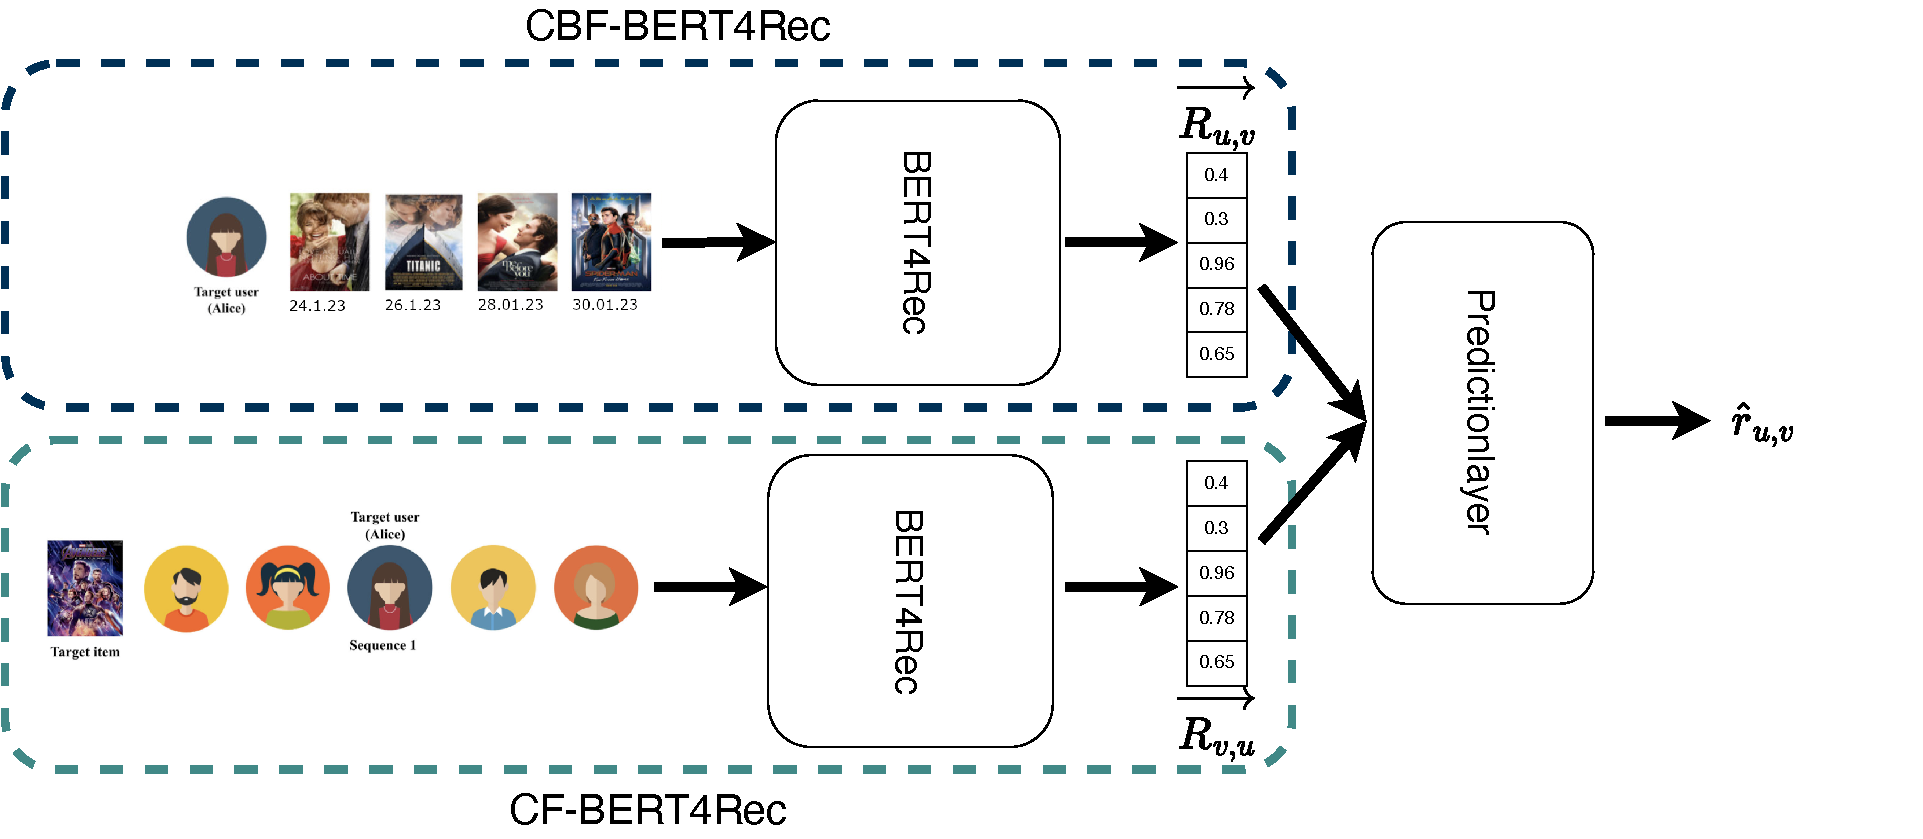
\includegraphics[height=0.6\textheight]{images/hybridBERT4Rec_high_level.pdf}
		\caption{High level overview of HybridBERT4Recs Architecture. \cite{channarongHybridBERT4RecHybridContentBased2022}}
	\end{figure}
\end{frame}
\begin{frame}{BERT4Rec \cite{sunBERT4RecSequentialRecommendation2019}}
	\begin{figure}
		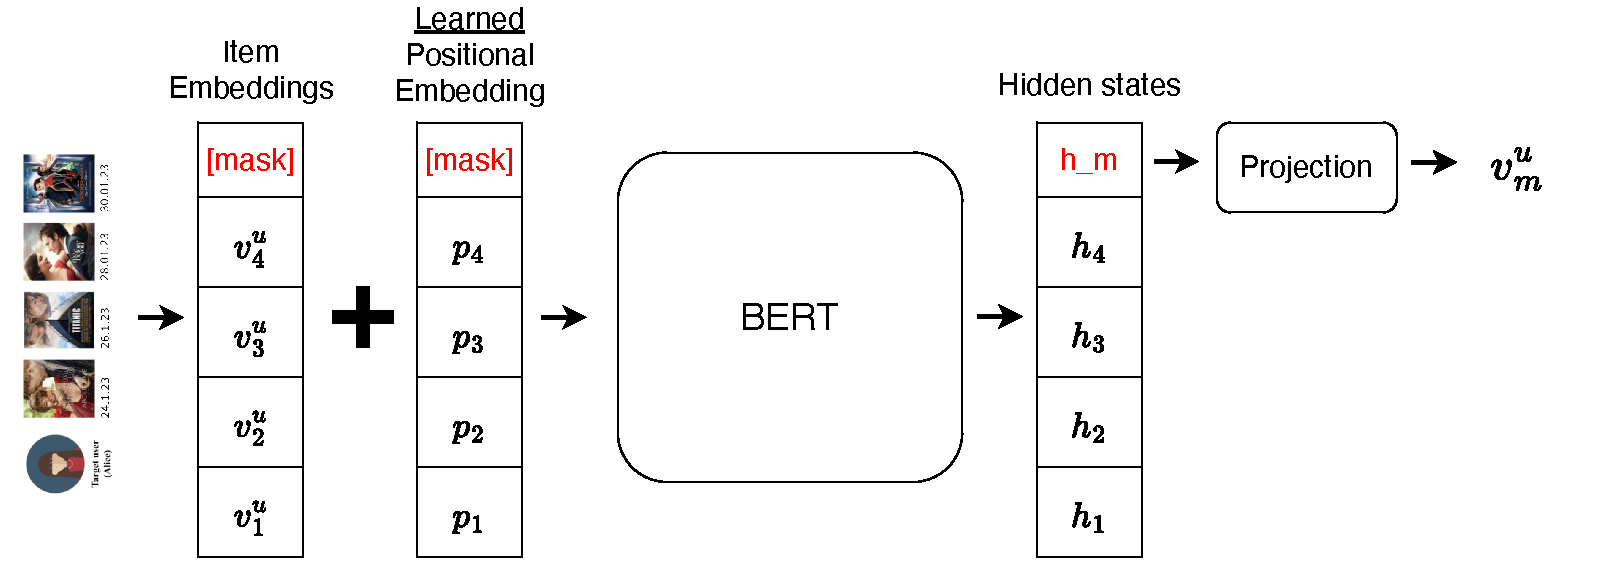
\includegraphics[width=0.9\textwidth]{images/BERT4Rec.pdf}
		\caption{BERT4Rec Architecture, taking item embeddings $v_t^u$ from user $u$ history as input and predicts the next item $v_m^u$, $u$ is likely to interact with. \cite{sunBERT4RecSequentialRecommendation2019}}
	\end{figure}
\end{frame}
\begin{frame}{CF-HybridBERT4Rec}
	\begin{figure}
		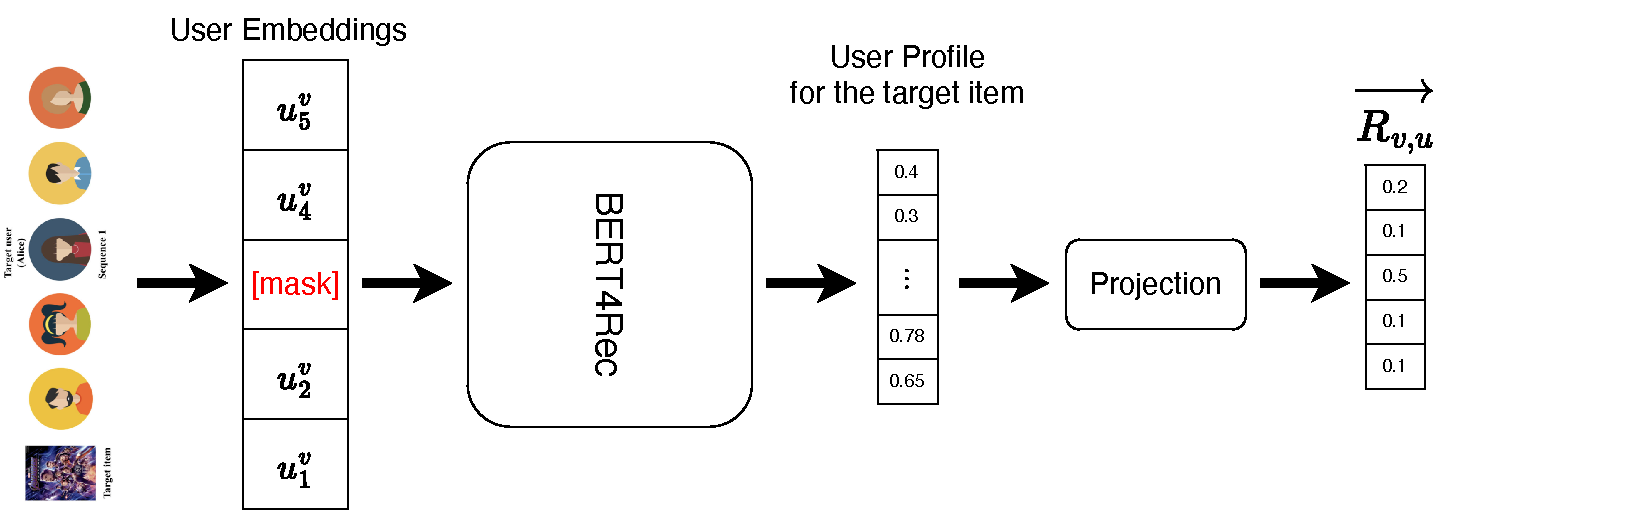
\includegraphics[width=0.9\textwidth]{images/CF-HybridBERT4Rec.pdf}
		\caption{CF-HybridBERT4Rec Architecture, taking user embeddings from all users that have rated the target item $v$ as input and predicts the \enquote{target item profile $\overrightarrow{R_{v,u}}$}. \cite{channarongHybridBERT4RecHybridContentBased2022}}
	\end{figure}
\end{frame}
\begin{frame}{CBF-HybridBERT4Rec}
	\begin{figure}
		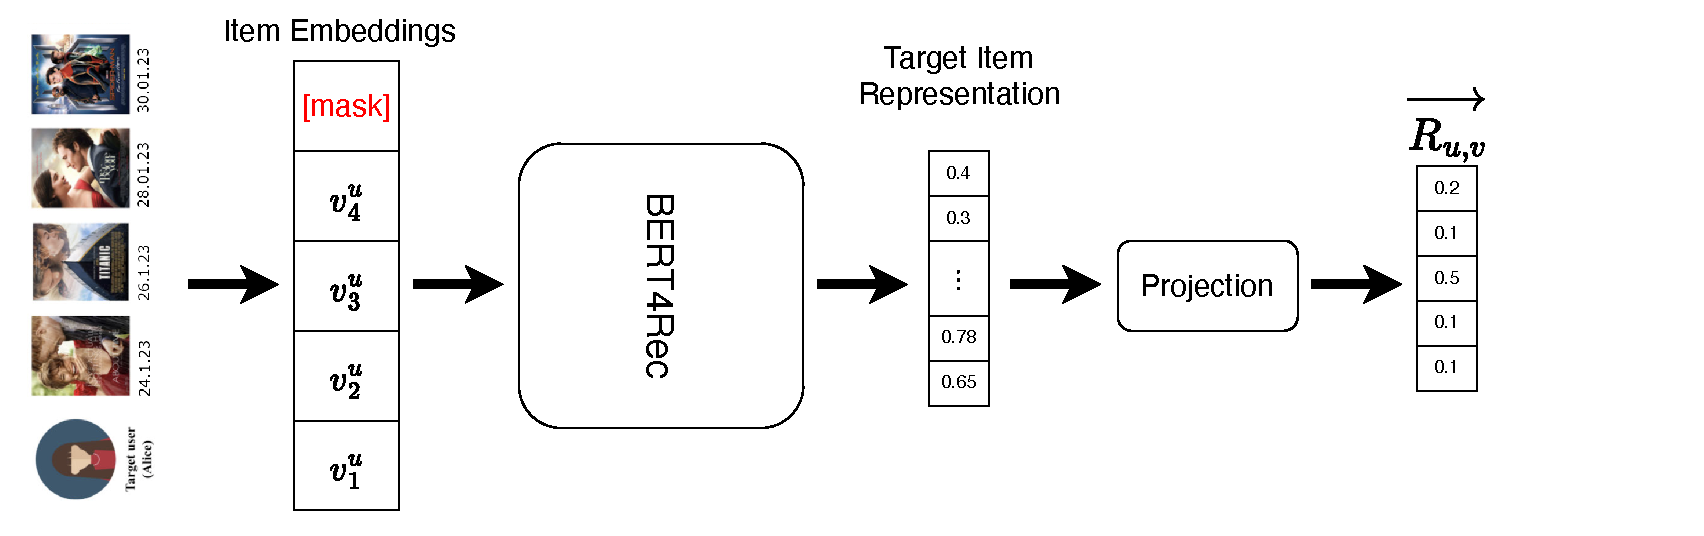
\includegraphics[width=0.9\textwidth]{images/CBF-HybridBERT4Rec.pdf}
		\caption{CBF-HybridBERT4Rec Architecture, taking item embeddings from a user $u$ history as input and predicts a \enquote{target user profile $\overrightarrow{R_{u,v}}$}. \cite{channarongHybridBERT4RecHybridContentBased2022}}
	\end{figure}
\end{frame}
\begin{frame}{Prediction Layer: Combining CF \& CBF}
	\begin{figure}
		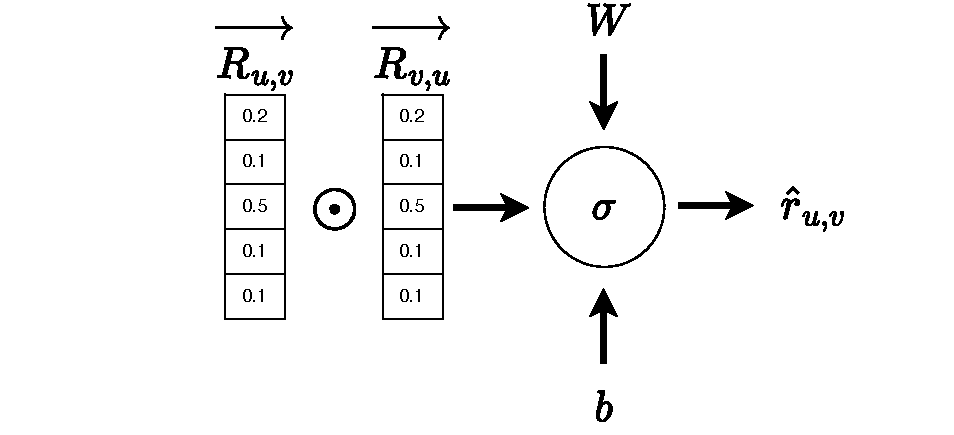
\includegraphics[height=0.5\textheight]{images/Prediction_Layer.pdf}
		\caption{Schematic of HybridBERT4Recs Prediction layer, which uses a generalization of Matrix Factorization based on Neural Networks with Sigmoid activations to predict the rating $\hat{r}_{u,v}$ user $u$ would assign to item $v$. \cite{channarongHybridBERT4RecHybridContentBased2022}}
	\end{figure}
\end{frame}

\subsection{Strengths \& Weaknesses}
\begin{frame}{Strengths \& Weaknesses}
	\begin{columns}
		\column[t]{.5\textwidth}
		\large{\textbf{Strengths:}}
		\begin{itemize}
			\item Easy to parallelize
			\item Bi-directional
			\item Sequential
			\item CBF-, CF-model \& Prediction layer can be executed independently
			\item Intermediate results can be cached
		\end{itemize}
		\column[t]{.5\textwidth}
		\large{\textbf{Weaknesses:}}
		\begin{itemize}
			\item Sequence length is limited
			\item Needs lots of processing power and memory
			\item Only uses rating information
		\end{itemize}
	\end{columns}
\end{frame}

\section{Model Performance \& Experiments}
\begin{frame}{Results}
	\begin{columns}
		\column{.6\textwidth}
		\begin{figure}
			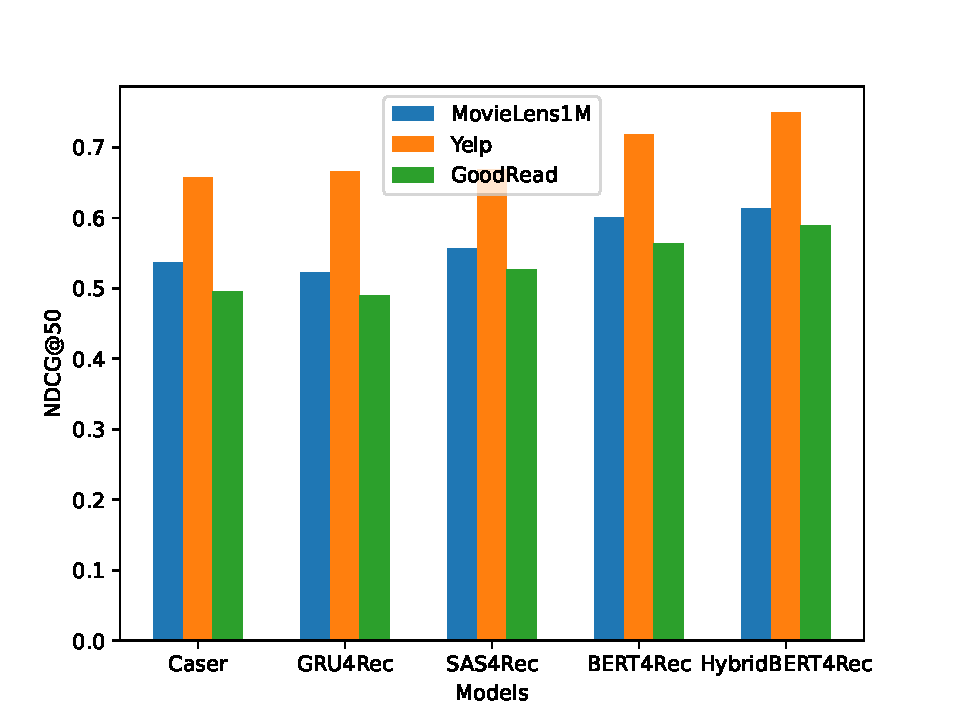
\includegraphics[height=0.55\textheight, width=0.8\textwidth]{images/results.pdf}
			\caption{Performance comparison of different recommender models on three datasets as published by the authors of HybridBERT4Rec. \cite{channarongHybridBERT4RecHybridContentBased2022}}
		\end{figure}
		\column{.4\textwidth}
		\textbf{Critique:}
		\begin{itemize} \pause
			\item No Hybrid model was evaluated!
			\item No information about data partitioning
			\item Generalization performance \& real world Applicability is unknown
		\end{itemize}
	\end{columns}
\end{frame}

\section{Applicability to E-Learning}
\begin{frame}{Applicability to E-Learning}
	\begin{columns}
		\column{0.5\textwidth}
		\begin{figure}
			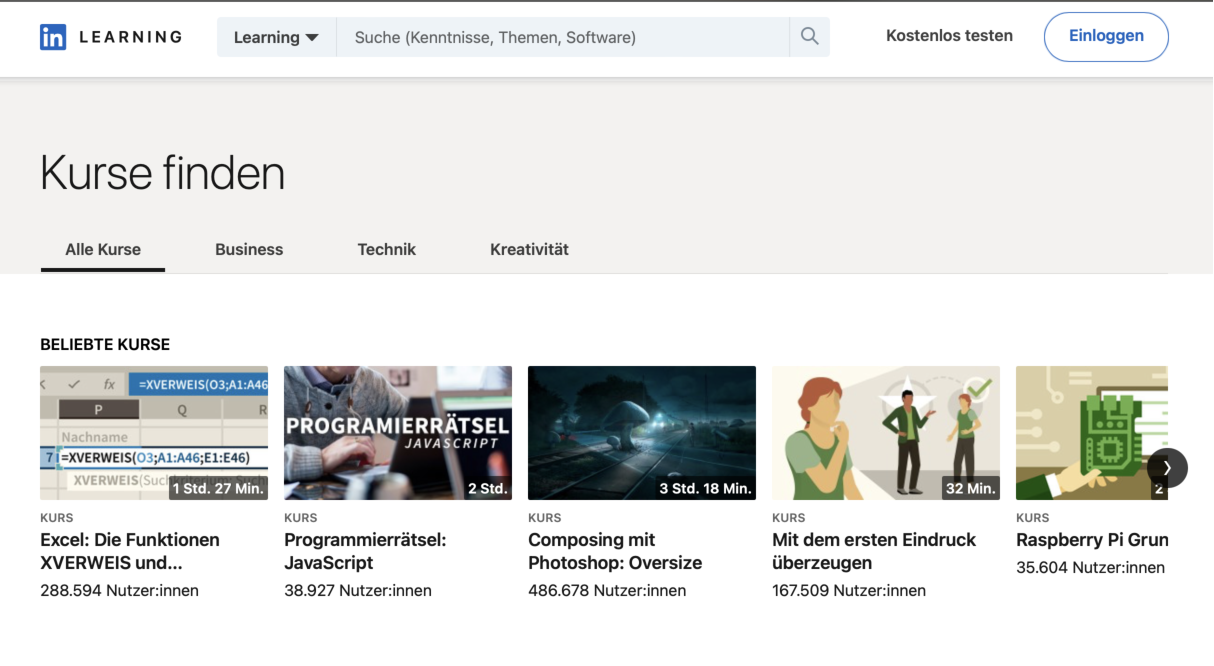
\includegraphics[height=0.55\textheight]{images/linked_in_landing.pdf}
			\caption{Linked-In Learning landing-page. \cite{LinkedInLearningMit}}
		\end{figure}
		\column{0.5\textwidth}
		\begin{figure}
			
\includegraphics[height=0.6\textheight]{images/linked_in_course.pdf}
			\caption{Linked-In Learning course overview. \cite{LinkedInLearningMit}}
		\end{figure}
	\end{columns}
\end{frame}

\appendix
\beginbackup
\begin{frame}{References}
	\printbibliography
\end{frame}
\backupend


% \subsection{Erster Unterabschnitt}
% \begin{frame}{Blöcke}{in den KIT-Farben}
% 	\begin{columns}
% 		\column{.3\textwidth}
% 		\begin{greenblock}{Greenblock}
% 			Standard (\texttt{block})
%         \end{greenblock}
% 		\column{.3\textwidth}
% 		\begin{blueblock}{Blueblock}
% 			= \texttt{exampleblock}
%         \end{blueblock}
% 		\column{.3\textwidth}
% 		\begin{redblock}{Redblock}
% 			= \texttt{alertblock}
%         \end{redblock}
% 	\end{columns}
% 	\begin{columns}
% 		\column{.3\textwidth}
%         \begin{brownblock}{Brownblock}
%         \end{brownblock}
% 		\column{.3\textwidth}
%         \begin{purpleblock}{Purpleblock}
%         \end{purpleblock}
% 		\column{.3\textwidth}
%         \begin{cyanblock}{Cyanblock}
%         \end{cyanblock}
% 	\end{columns}
% 	\begin{columns}
% 		\column{.3\textwidth}
%         \begin{yellowblock}{Yellowblock}
%         \end{yellowblock}
% 		\column{.3\textwidth}
%         \begin{lightgreenblock}{Lightgreenblock}
%         \end{lightgreenblock}
% 		\column{.3\textwidth}
%         \begin{orangeblock}{Orangeblock}
%         \end{orangeblock}
% 	\end{columns}
% 	\begin{columns}
% 		\column{.3\textwidth}
%         \begin{grayblock}{Grayblock}
%         \end{grayblock}
% 		\column{.3\textwidth}
% 		\begin{contentblock}{Contentblock}
% 			(farblos)
% 		\end{contentblock}
% 		\column{.3\textwidth}
% 	\end{columns}
% \end{frame}
	  
% \subsection{Zweiter Unterabschnitt}
% \begin{frame}{Auflistungen}
% 	Text
% 	\begin{itemize}
% 		\item Auflistung\\ Umbruch
% 		\item Auflistung
% 		\begin{itemize}
% 			\item Auflistung
% 			\item Auflistung
% 		\end{itemize}
% 	\end{itemize}
% \end{frame}

% \section{Zweiter Abschnitt}

% \begin{frame}
%         Bei Frames ohne Titel wird die Kopfzeile nicht angezeigt, und  
%     der freie Platz kann für Inhalte genutzt werden.
% \end{frame}

% \begin{frame}[plain]
%     Bei Frames mit Option \texttt{[plain]} werden weder Kopf- noch Fußzeile angezeigt.
% \end{frame}

% \begin{frame}[t]{Beispielinhalt}
%     Bei Frames mit Option \texttt{[t]} werden die Inhalte nicht vertikal zentriert, sondern an der Oberkante begonnen.
% \end{frame}


% \begin{frame}{Beispielinhalt: Literatur}
%     Literaturzitat: \cite{klare2021jss}
% \end{frame}

% \appendix
% \beginbackup

% \begin{frame}{Literatur}
% \begin{exampleblock}{Backup-Teil}
%     Folien, die nach \texttt{\textbackslash beginbackup} eingefügt werden, zählen nicht in die Gesamtzahl der Folien.
% \end{exampleblock}

% \printbibliography
% \end{frame}

% \section{Farben}
% %% ----------------------------------------
% %% | Test-Folie mit definierten Farben |
% %% ----------------------------------------
% \begin{frame}{Farbpalette}
% \tiny

% % GREEN
% 	\colorbox{kit-green100}{kit-green100}
% 	\colorbox{kit-green90}{kit-green90}
% 	\colorbox{kit-green80}{kit-green80}
% 	\colorbox{kit-green70}{kit-green70}
% 	\colorbox{kit-green60}{kit-green60}
% 	\colorbox{kit-green50}{kit-green50}
% 	\colorbox{kit-green40}{kit-green40}
% 	\colorbox{kit-green30}{kit-green30}
% 	\colorbox{kit-green25}{kit-green25}
% 	\colorbox{kit-green20}{kit-green20}
% 	\colorbox{kit-green15}{kit-green15}
% 	\colorbox{kit-green10}{kit-green10}
% 	\colorbox{kit-green5}{kit-green5}

% % BLUE
% 	\colorbox{kit-blue100}{kit-blue100}
% 	\colorbox{kit-blue90}{kit-blue90}
% 	\colorbox{kit-blue80}{kit-blue80}
% 	\colorbox{kit-blue70}{kit-blue70}
% 	\colorbox{kit-blue60}{kit-blue60}
% 	\colorbox{kit-blue50}{kit-blue50}
% 	\colorbox{kit-blue40}{kit-blue40}
% 	\colorbox{kit-blue30}{kit-blue30}
% 	\colorbox{kit-blue25}{kit-blue25}
% 	\colorbox{kit-blue20}{kit-blue20}
% 	\colorbox{kit-blue15}{kit-blue15}
% 	\colorbox{kit-blue10}{kit-blue10}
% 	\colorbox{kit-blue5}{kit-blue5}

% % RED
% 	\colorbox{kit-red100}{kit-red100}
% 	\colorbox{kit-red90}{kit-red90}
% 	\colorbox{kit-red80}{kit-red80}
% 	\colorbox{kit-red70}{kit-red70}
% 	\colorbox{kit-red60}{kit-red60}
% 	\colorbox{kit-red50}{kit-red50}
% 	\colorbox{kit-red40}{kit-red40}
% 	\colorbox{kit-red30}{kit-red30}
% 	\colorbox{kit-red25}{kit-red25}
% 	\colorbox{kit-red20}{kit-red20}
% 	\colorbox{kit-red15}{kit-red15}
% 	\colorbox{kit-red10}{kit-red10}
% 	\colorbox{kit-red5}{kit-red5}

% % GREY
% 	\colorbox{kit-gray100}{\color{white}kit-gray100}
% 	\colorbox{kit-gray90}{\color{white}kit-gray90}
% 	\colorbox{kit-gray80}{\color{white}kit-gray80}
% 	\colorbox{kit-gray70}{\color{white}kit-gray70}
% 	\colorbox{kit-gray60}{\color{white}kit-gray60}
% 	\colorbox{kit-gray50}{\color{white}kit-gray50}
% 	\colorbox{kit-gray40}{kit-gray40}
% 	\colorbox{kit-gray30}{kit-gray30}
% 	\colorbox{kit-gray25}{kit-gray25}
% 	\colorbox{kit-gray20}{kit-gray20}
% 	\colorbox{kit-gray15}{kit-gray15}
% 	\colorbox{kit-gray10}{kit-gray10}
% 	\colorbox{kit-gray5}{kit-gray5}

% % Orange
% 	\colorbox{kit-orange100}{kit-orange100}
% 	\colorbox{kit-orange90}{kit-orange90}
% 	\colorbox{kit-orange80}{kit-orange80}
% 	\colorbox{kit-orange70}{kit-orange70}
% 	\colorbox{kit-orange60}{kit-orange60}
% 	\colorbox{kit-orange50}{kit-orange50}
% 	\colorbox{kit-orange40}{kit-orange40}
% 	\colorbox{kit-orange30}{kit-orange30}
% 	\colorbox{kit-orange25}{kit-orange25}
% 	\colorbox{kit-orange20}{kit-orange20}
% 	\colorbox{kit-orange15}{kit-orange15}
% 	\colorbox{kit-orange10}{kit-orange10}
% 	\colorbox{kit-orange5}{kit-orange5}

% % lightgreen
% 	\colorbox{kit-lightgreen100}{kit-lightgreen100}
% 	\colorbox{kit-lightgreen90}{kit-lightgreen90}
% 	\colorbox{kit-lightgreen80}{kit-lightgreen80}
% 	\colorbox{kit-lightgreen70}{kit-lightgreen70}
% 	\colorbox{kit-lightgreen60}{kit-lightgreen60}
% 	\colorbox{kit-lightgreen50}{kit-lightgreen50}
% 	\colorbox{kit-lightgreen40}{kit-lightgreen40}
% 	\colorbox{kit-lightgreen30}{kit-lightgreen30}
% 	\colorbox{kit-lightgreen25}{kit-lightgreen25}
% 	\colorbox{kit-lightgreen20}{kit-lightgreen20}
% 	\colorbox{kit-lightgreen15}{kit-lightgreen15}
% 	\colorbox{kit-lightgreen10}{kit-lightgreen10}
% 	\colorbox{kit-lightgreen5}{kit-lightgreen5}

% % Brown
% 	\colorbox{kit-brown100}{kit-brown100}
% 	\colorbox{kit-brown90}{kit-brown90}
% 	\colorbox{kit-brown80}{kit-brown80}
% 	\colorbox{kit-brown70}{kit-brown70}
% 	\colorbox{kit-brown60}{kit-brown60}
% 	\colorbox{kit-brown50}{kit-brown50}
% 	\colorbox{kit-brown40}{kit-brown40}
% 	\colorbox{kit-brown30}{kit-brown30}
% 	\colorbox{kit-brown25}{kit-brown25}
% 	\colorbox{kit-brown20}{kit-brown20}
% 	\colorbox{kit-brown15}{kit-brown15}
% 	\colorbox{kit-brown10}{kit-brown10}
% 	\colorbox{kit-brown5}{kit-brown5}

% % Purple
% 	\colorbox{kit-purple100}{kit-purple100}
% 	\colorbox{kit-purple90}{kit-purple90}
% 	\colorbox{kit-purple80}{kit-purple80}
% 	\colorbox{kit-purple70}{kit-purple70}
% 	\colorbox{kit-purple60}{kit-purple60}
% 	\colorbox{kit-purple50}{kit-purple50}
% 	\colorbox{kit-purple40}{kit-purple40}
% 	\colorbox{kit-purple30}{kit-purple30}
% 	\colorbox{kit-purple25}{kit-purple25}
% 	\colorbox{kit-purple20}{kit-purple20}
% 	\colorbox{kit-purple15}{kit-purple15}
% 	\colorbox{kit-purple10}{kit-purple10}
% 	\colorbox{kit-purple5}{kit-purple5}

% % Cyan
% 	\colorbox{kit-cyan100}{kit-cyan100}
% 	\colorbox{kit-cyan90}{kit-cyan90}
% 	\colorbox{kit-cyan80}{kit-cyan80}
% 	\colorbox{kit-cyan70}{kit-cyan70}
% 	\colorbox{kit-cyan60}{kit-cyan60}
% 	\colorbox{kit-cyan50}{kit-cyan50}
% 	\colorbox{kit-cyan40}{kit-cyan40}
% 	\colorbox{kit-cyan30}{kit-cyan30}
% 	\colorbox{kit-cyan25}{kit-cyan25}
% 	\colorbox{kit-cyan20}{kit-cyan20}
% 	\colorbox{kit-cyan15}{kit-cyan15}
% 	\colorbox{kit-cyan10}{kit-cyan10}
% 	\colorbox{kit-cyan5}{kit-cyan5}
		
% \end{frame}
% %% ----------------------------------------
% %% | /Test-Folie mit definierten Farben |
% %% ----------------------------------------
% \backupend

\end{document}